%================================================================
% 作業ログ 2026-06-30（本番プログラム構築・テスト検証基盤・筐体モデリング）
%   production フォルダ新設＋バグ修正・実機テスト後修正，
%   MOE/MOP 検証プログラム作成，3Dプリンタ用筐体モデリング．
%
%   ビルド:
%     cd work/shiozawa/work-0630/作業ログ0630
%     docker run --rm -v "$(pwd):/workspace" -w /workspace \
%       ghcr.io/paperist/texlive-ja:debian latexmk 作業ログ0630.tex
%================================================================
\documentclass[uplatex,dvipdfmx,a4paper,11pt]{jsarticle}

% --- 余白 ---
\usepackage[top=25mm,bottom=25mm,left=25mm,right=25mm]{geometry}

% --- 表・箇条書き・図・色 ---
\usepackage{array}
\usepackage{tabularx}
\usepackage{booktabs}
\usepackage{enumitem}
\usepackage{graphicx}
\usepackage{url}
\usepackage[table]{xcolor}
\usepackage{amssymb}

% --- 段落間隔（Wordのような見た目に寄せる）---
\setlength{\parindent}{0pt}
\setlength{\parskip}{0.6em}

% --- セクション見出しを「番号. 太字」+ 章末に水平線を入れる ---
\usepackage{titlesec}
\titleformat{\section}
  {\normalfont\Large\bfseries}{\thesection.}{0.6em}{}
\titleformat{\subsection}
  {\normalfont\large\bfseries}{\thesubsection}{0.6em}{}
\titlespacing*{\section}{0pt}{1.2em}{0.6em}
\titlespacing*{\subsection}{0pt}{1.0em}{0.4em}

% --- 章末水平線（手で \sectionrule と書いて区切る）---
\newcommand{\sectionrule}{\par\medskip\noindent\rule{\linewidth}{0.6pt}\par\medskip}

% --- 箇条書きの記号を Word 風（・→○→数字）に揃える ---
\renewcommand{\labelitemi}{\textbullet}
\renewcommand{\labelitemii}{\textopenbullet}
\setlist[itemize]{leftmargin=1.6em,itemsep=0.1em,topsep=0.2em}
\setlist[enumerate]{leftmargin=2.0em,itemsep=0.1em,topsep=0.2em}

% \textopenbullet が無い環境向けのフォールバック
\providecommand{\textopenbullet}{\ensuremath{\circ}}

% --- 進捗ガントチャート用（グリッド表）---
\definecolor{barDone}{gray}{0.55} % 完了
\definecolor{barProg}{gray}{0.78} % 進行中
\definecolor{barPlan}{gray}{0.90} % 予定
\definecolor{nowCol}{gray}{0.30}  % 今週の見出し
\newcolumntype{G}{>{\centering\arraybackslash}p{2.0em}}
\newcommand{\bD}{\cellcolor{barDone}}
\newcommand{\bP}{\cellcolor{barProg}}
\newcommand{\bQ}{\cellcolor{barPlan}}

\begin{document}

%================================================================
% ヘッダ
%================================================================
{\LARGE\bfseries 作業ログ}\par\bigskip

報告者：塩澤 匠生

報告日：2026年6月30日

プロジェクト名：タクトーン~ IMUジェスチャーで奏でるArduinoオーケストラ~ \\

\sectionrule

%================================================================
% 1. 進捗サマリー
%================================================================
\section{進捗サマリー（要約）}

\begin{itemize}
  \item 全体進捗率：90\%（先週 70\% → 90\%．本番プログラム構築・実機テスト・
        バグ修正を集中的に実施し，発表会デモ可能な状態に到達）
  \item 進捗状況（今週の変化）：
    \begin{itemize}
      \item production フォルダを新設し，本番用ファーム＋Processing を分離（全 7 ノード）
      \item 実機テスト後のバグ修正を複数回実施（PR \#27〜\#32，計 30 件超の修正）
      \item MOE/MOP 全 9 項目の検証プログラムを新規作成（Python スクリプト＋検証ファーム）
      \item マルチ Arduino テストダッシュボード＋Processing 共通ライブラリを作成
      \item 3D プリンタ用の指揮棒筐体を CAD でモデリング
    \end{itemize}
  \item 今週の主要成果：
    \begin{itemize}
      \item 本番環境（production）が実機で動作する状態になった
      \item 評価項目（MOE/MOP）を自動検証できる基盤が整った
      \item 指揮棒の筐体設計が完了し，3D プリント待ちの状態
    \end{itemize}
  \item 重大課題（影響度：低）：
    \begin{itemize}
      \item {}[発表会（7/8）に向け，残りはデモ構成の最終調整のみ]
    \end{itemize}
\end{itemize}

\sectionrule

%================================================================
% 2. 進捗ガントチャート（計画と現在地）
%================================================================
\section{進捗ガントチャート（計画と現在地）}

チームのガントチャート（\texttt{meetings/ガントチャーver1ト.xlsx}）のフェーズ区分（110 基本設計／
120 詳細設計／200 実装／300 テスト／400 ストレッチ）に，現在の進み具合を重ねたもの．
「今」の縦位置は本報告時点（7 月第 1 週＝発表会）．

\medskip
{\footnotesize
\setlength{\tabcolsep}{2pt}
\renewcommand{\arraystretch}{1.2}
\begin{tabular}{@{}p{8.5em}|*{12}{G}@{}}
 & & & & & & & & & & & & \multicolumn{1}{c}{$\downarrow$今} \\
作業項目（フェーズ）
 & \cellcolor{barPlan}\tiny 4/15 & \cellcolor{barPlan}\tiny 4/22 & \cellcolor{barPlan}\tiny 4/29
 & \cellcolor{barPlan}\tiny 5/6 & \cellcolor{barPlan}\tiny 5/13 & \cellcolor{barPlan}\tiny 5/20
 & \cellcolor{barPlan}\tiny 5/27 & \cellcolor{barPlan}\tiny 6/3 & \cellcolor{barPlan}\tiny 6/10
 & \cellcolor{barPlan}\tiny 6/17 & \cellcolor{barPlan}\tiny 6/24 & \cellcolor{nowCol}\tiny\textcolor{white}{7/8} \\
\midrule
企画・テーマ決定        & \bD & \bD &     &     &     &     &     &     &     &     &     &     \\
110 基本設計            &     &     & \bD & \bD &     &     &     &     &     &     &     &     \\
120 詳細設計            &     &     &     &     & \bD &     &     &     &     &     &     &     \\
\textbf{200 実装}       &     &     &     &     &     &     &     &     &     &     &     &     \\
\quad test\_v2 輪唱・同期 &     &     &     & \bD & \bD & \bD & \bD &     &     &     &     &     \\
\quad test\_v3 ゲーム(firmware) &  &     &     &     &     & \bD & \bD & \bD & \bD &     &     &     \\
\quad test\_v3 Processing &   &     &     &     &     &     & \bD & \bD & \bD &     &     &     \\
\quad production 構築    &     &     &     &     &     &     &     &     &     &     & \bD & \bD \\
\textbf{300 テスト}     &     &     &     &     &     &     &     &     &     &     &     &     \\
\quad 単体・結合・システム &   &     &     &     &     &     &     &     & \bD & \bD & \bD &     \\
\quad 評価（精度・遅延） &     &     &     &     &     &     &     &     &     &     & \bD & \bP \\
400 ストレッチ（強弱ほか） &  &     &     &     &     &     &     & \bQ & \bQ &     &     &     \\
発表会                  &     &     &     &     &     &     &     &     &     &     &     & \multicolumn{1}{c}{$\bigstar$} \\
\bottomrule
\end{tabular}
}

\medskip
凡例：\colorbox{barDone}{~~}~完了 \quad \colorbox{barProg}{~~}~進行中 \quad
\colorbox{barPlan}{~~}~予定 \quad $\bigstar$~発表会（7/8）

\medskip
※ 今週は本番プログラム（production）の構築・実機テスト・バグ修正に集中．
評価（MOE/MOP 検証プログラム）の基盤も整備完了．来週の発表会（7/8）に向けた最終調整段階．

\sectionrule

%================================================================
% 3. 作業ログ（詳細トラッキング）
%================================================================
\section{作業ログ（詳細トラッキング）}

\begin{tabularx}{\linewidth}{@{}p{10em}p{6em}p{4em}p{3em}X@{}}
\toprule
作業項目 & 実施日 & 作業時間 & 進捗 & コメント \\
\midrule
production フォルダ新設 & 2026-06-24 & 15 分 & 100\% & test\_v3 ベースの本番用コードを production フォルダに分離（全 7 ノード） \\
production Processing 修正 & 2026-06-24 & 30 分 & 100\% & オクターブ移調・音揺れ・ドラム合成周波数・チューバ音域/音量を齋藤版に準拠して修正（PR \#27〜\#29） \\
実機テスト後の修正 & 2026-06-24 & 20 分 & 100\% & ナビゲート復帰・ドラム楽譜簡素化・Fallback 無効化・感度パラメータ復元（PR \#30, \#31） \\
production バグ修正 & 2026-06-25 & 25 分 & 100\% & 19 件のバグ修正＋リファクタ＋通信改善（PR \#32） \\
テストダッシュボード作成 & 2026-06-25 & 15 分 & 100\% & マルチ Arduino テストダッシュボード＋Processing 共通ライブラリ（PR \#33） \\
MOE/MOP 検証プログラム & 2026-06-25 & 10 分 & 100\% & serial\_logger.py（複数ポート同時ログ）＋analyze.py（9 項目 PASS/FAIL 判定）＋検証ファーム \\
ゲーム UI 改善 & 2026-06-28 & 5 分 & 100\% & test\_multi 指揮者パネルを production 版ゲーム UI に変更 \\
\midrule
\multicolumn{2}{@{}l}{\textbf{ソフトウェア 小計}} & \textbf{120 分} & & \\
\midrule
指揮棒筐体モデリング & 2026-06-29 & 120 分 & 100\% & 3D CAD で指揮者マイコン（Arduino UNO R4 WiFi + IMU）を収める筐体を設計．角にフィレット，USB 用開口部，蓋と本体の嵌合構造 \\
\midrule
\multicolumn{2}{@{}l}{\textbf{合計}} & \textbf{240 分} & & \\
\bottomrule
\end{tabularx}

\sectionrule

%================================================================
% 4. 課題管理
%================================================================
\section{課題管理}

\begin{tabularx}{\linewidth}{@{}p{8em}Xp{2.5em}p{2.5em}Xp{3em}@{}}
\toprule
課題 & 発生原因 & 影響度 & 優先度 & 対策 & 状態 \\
\midrule
マイコン破損 & 前週の配線ミス & 高 & 高 & 代替品到着後ソケットに載せ替え，正常動作を確認 & 解決済 \\
production バグ多発 & test\_v3 からの移行時に不整合 & 中 & 高 & PR \#27〜\#32 で計 30 件超を修正し安定化 & 解決済 \\
\bottomrule
\end{tabularx}

\medskip
※影響度＝プロジェクトへのインパクト，優先度＝対応の緊急性

\sectionrule

%================================================================
% 5. AI利用状況と検証
%================================================================
\section{AI利用状況と検証(再現性重視)}

\subsection{利用内容}

\begin{itemize}
  \item Claude Code を用いて production のバグ修正・リファクタ・テストダッシュボード作成・
        MOE/MOP 検証プログラム作成を実施
  \item 具体的には PR \#32（バグ修正 19 件），PR \#33（テストダッシュボード），
        MOE/MOP 検証スクリプト（serial\_logger.py, analyze.py）の生成を支援
  \item 生成コードは \texttt{pio run} でビルド成功を確認し，実機テストで動作検証済み
\end{itemize}

\sectionrule

%================================================================
% 6. 次回計画
%================================================================
\section{次回計画}

\begin{itemize}
  \item 目標：
    \begin{itemize}
      \item {}[7/8 発表会でデモを成功させる]
      \item {}[MOE/MOP 検証プログラムで最終評価を実施する]
    \end{itemize}
  \item 達成基準：
    \begin{itemize}
      \item {}[発表会で指揮→楽器→PC の一連の流れが正常に動作する]
      \item {}[MOE/MOP 9 項目のうち必達項目がすべて PASS する]
    \end{itemize}
  \item 期限：
    \begin{itemize}
      \item {}[7/8 発表会当日]
    \end{itemize}
\end{itemize}

\sectionrule

%================================================================
% 7. その他
%================================================================
\section{その他}

\begin{itemize}
  \item {}[今週は本番プログラム（production）の構築と安定化に集中した．
        test\_v3 から production への分離後に多数のバグが見つかったが，
        PR \#27〜\#32 の集中修正で安定した状態になった]
  \item {}[MOE/MOP 全 9 項目の検証プログラムを作成し，評価を自動化できる
        基盤が整った．serial\_logger.py で複数ポートのログを同時収集し，
        analyze.py で PASS/FAIL を自動判定する]
  \item {}[3D プリンタ用の指揮棒筐体を CAD でモデリングした．
        Arduino UNO R4 WiFi と IMU を収める長方形ケースで，角にフィレット，
        USB コネクタ用の開口部，蓋固定用のネジ穴を設けた]
  \item {}[来週が発表会（7/8）．本番環境は動作確認済みで，
        デモ構成の最終調整のみ残っている状態]
\end{itemize}

\sectionrule

%================================================================
% 8. 付録
%================================================================
\section{付録}

\begin{itemize}
  \item 添付資料：
    \begin{itemize}
      \item GitHub リポジトリ：\url{https://github.com/takushio2525/2026-hackathon-team23}
      \item 筐体 3D モデル：図\ref{fig:case-outer}（外観），図\ref{fig:case-inner}（内部）
    \end{itemize}
  \item 主要コミット（塩澤担当分）：
    \begin{itemize}
      \item \texttt{c1db8e3} --- 本番プログラム production フォルダ新設（PR \#26）
      \item \texttt{4d1e051} --- production バグ修正 19 件＋リファクタ＋通信改善（PR \#32）
      \item \texttt{eea3df2} --- マルチ Arduino テストダッシュボード＋Processing 共通ライブラリ（PR \#33）
      \item \texttt{f3fddc6} --- MOE/MOP 全 9 項目の検証プログラムを新規作成
      \item \texttt{1f33943} --- test\_multi 指揮者パネルを production 版ゲーム UI に変更
    \end{itemize}
\end{itemize}

\bigskip

% --- 筐体 3D モデル ---
\begin{figure}[h]
  \centering
  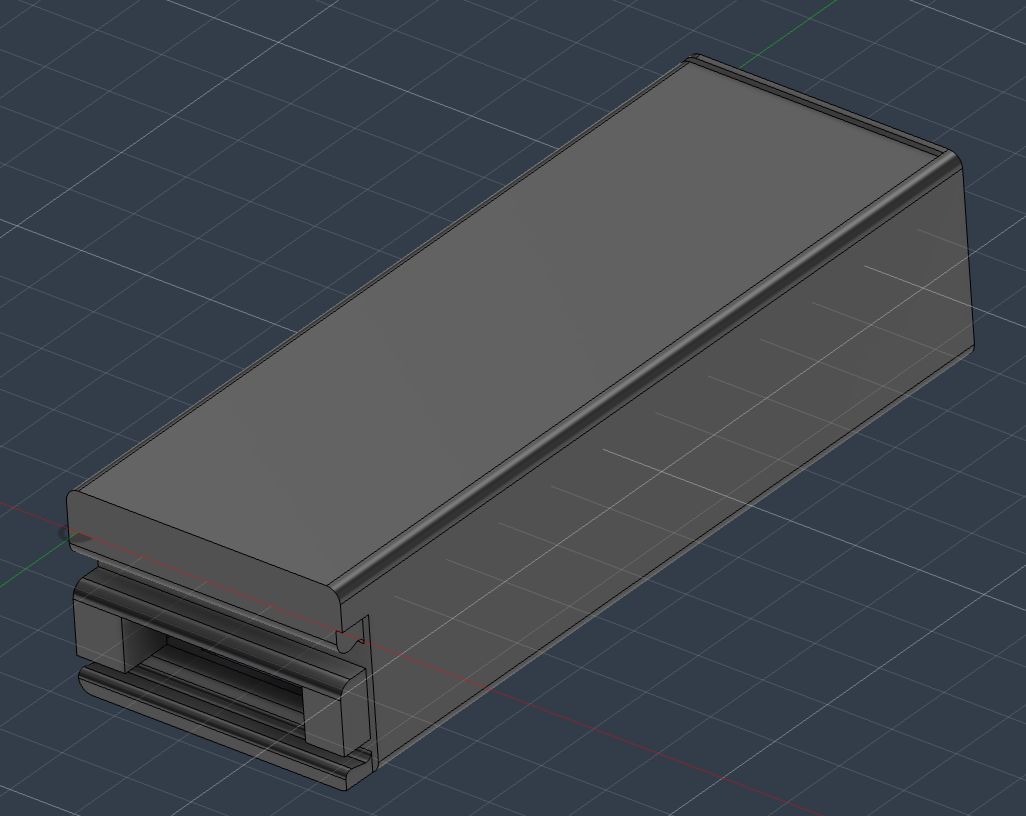
\includegraphics[width=0.7\linewidth]{fig/case_outer.png}
  \caption{指揮棒筐体 3D モデル（外観）：角にフィレット，一端に USB コネクタ用の開口部}
  \label{fig:case-outer}
\end{figure}

\begin{figure}[h]
  \centering
  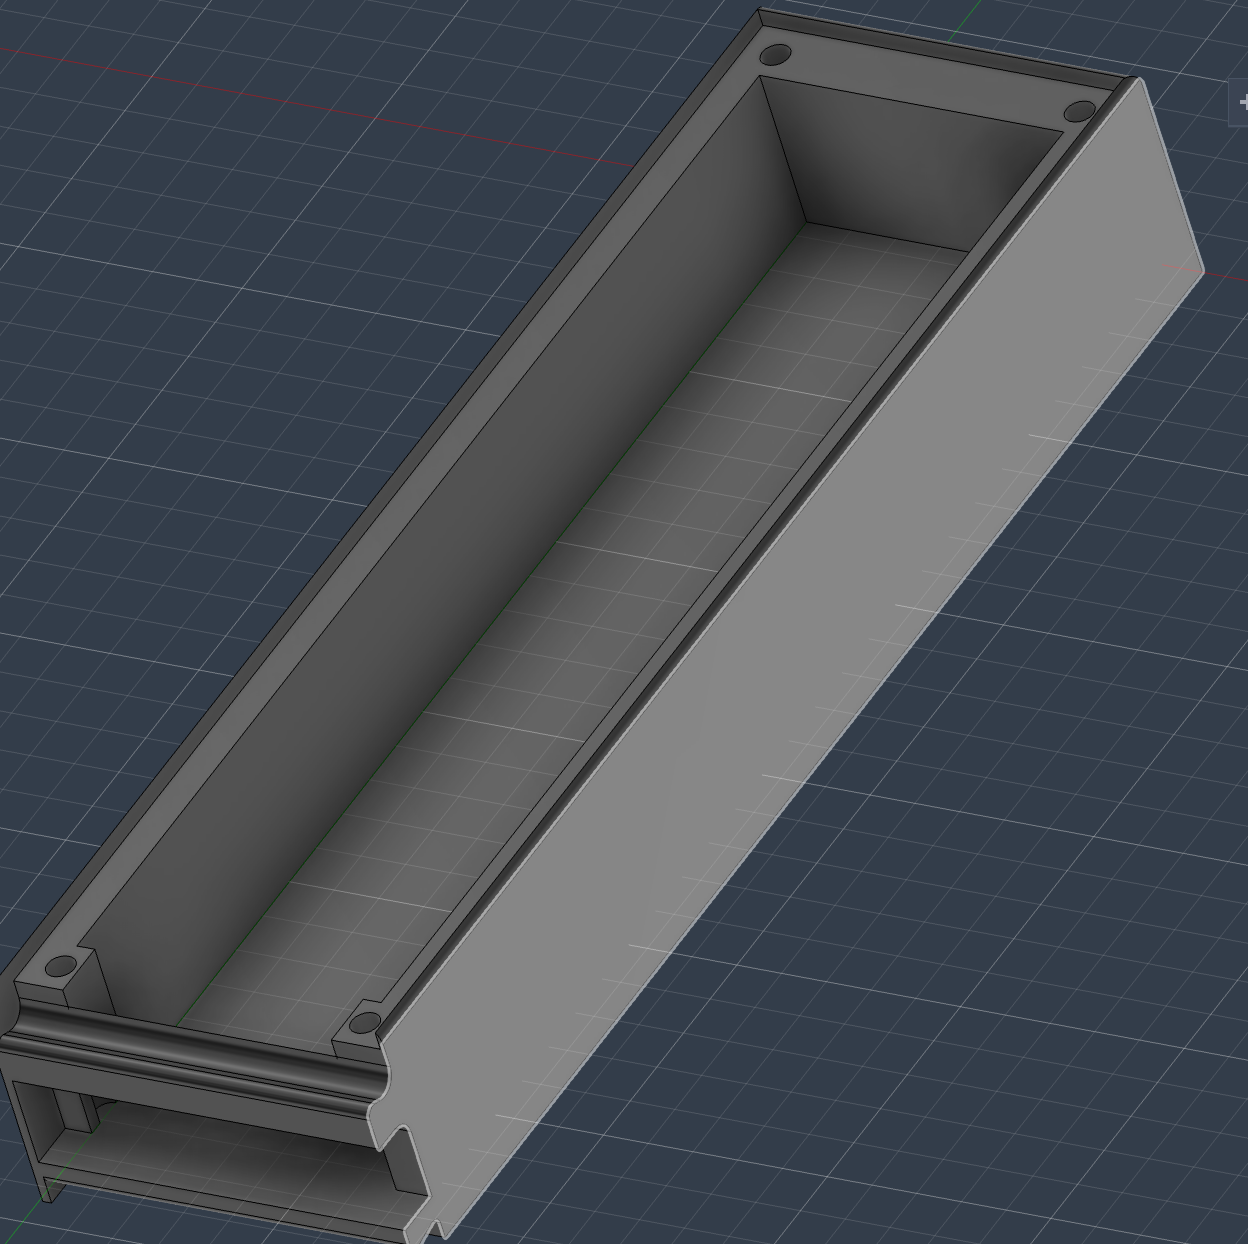
\includegraphics[width=0.7\linewidth]{fig/case_inner.png}
  \caption{指揮棒筐体 3D モデル（内部）：四隅にネジ穴，蓋と本体の嵌合構造}
  \label{fig:case-inner}
\end{figure}

\sectionrule

\end{document}
